\documentclass[a4paper]{article}

%% Language and font encodings
\usepackage[french]{babel}
\usepackage[utf8]{inputenc}
\usepackage[T1]{fontenc}

\usepackage{float}

\setlength{\parindent}{1em}
%\setlength{\parskip}{1ex plus 0.5ex minus 0.2ex}
\newcommand{\hsp}{\hspace{20pt}}
\newcommand{\HRule}{\rule{\linewidth}{0.5mm}}

\usepackage{algorithm}
\usepackage[noend]{algpseudocode}
\algnewcommand{\algorithmicand}{\textbf{ and }}
\algnewcommand{\algorithmicor}{\textbf{ or }}
\algnewcommand{\OR}{\algorithmicor}
\algnewcommand{\AND}{\algorithmicand}
\algnewcommand\algorithmicforeach{\textbf{for each}}
\algdef{S}[FOR]{ForEach}[1]{\algorithmicforeach\ #1\ \algorithmicdo}
\newcommand{\myfrac}[2]{\frac{\displaystyle {#1}}{\displaystyle {#2}}}

%% Sets page size and margins
\usepackage[a4paper,top=3cm,bottom=2cm,left=3cm,right=3cm,marginparwidth=1.75cm]{geometry}

%% Useful packages
\usepackage{amsmath}
\usepackage{amssymb}
\usepackage{graphicx}
\usepackage{subcaption}
\usepackage[colorinlistoftodos]{todonotes}
\usepackage[colorlinks=true, allcolors=blue]{hyperref}
\usepackage{graphicx}

\usepackage{enumitem}

\usepackage{listings}
\lstset{language=Python} 

\usepackage[htt]{hyphenat}

%% equations
\usepackage{amsthm}
\usepackage[retainorgcmds]{IEEEtrantools}

%% theorem and proposition
\newtheorem{prop}{Proposition}
\newtheorem*{prop*}{Proposition}
\newtheorem{thm}{Théorème}

\newenvironment{myproof}[1][\proofname]{\proof[#1]\mbox{}\\*}{\endproof}

%% references shortcuts (Arthur) 
\usepackage{suffix}
\renewcommand{\eqref}[1]{équation~\ref{#1}}
\newcommand{\algoref}[1]{algorithme~\ref{#1}}
\newcommand{\figref}[1]{figure~\ref{#1}}
\newcommand{\tabref}[1]{tableau~\ref{#1}}
\newcommand{\secref}[1]{section~\ref{#1}}
\newcommand{\probref}[1]{problème~\ref{#1}}
\newcommand{\propref}[1]{proposition~\ref{#1}}
\newcommand{\theoremref}[1]{théorème~\ref{#1}}
\newcommand{\chapref}[1]{chapitre~\ref{#1}}
\newcommand{\appref}[1]{annexe~\ref{#1}}
\WithSuffix\newcommand\algoref*[1]{algorithme~\ref{#1} p.~\pageref{#1}}
\WithSuffix\newcommand\figref*[1]{figure~\ref{#1} p.~\pageref{#1}}
\WithSuffix\newcommand\eqref*[1]{équation~\ref{#1} p.~\pageref{#1}}
\WithSuffix\newcommand\tabref*[1]{tableau~\ref{#1} p.~\pageref{#1}}
\WithSuffix\newcommand\secref*[1]{section~\ref{#1} p.~\pageref{#1}}
\WithSuffix\newcommand\probref*[1]{problème~\ref{#1} p.~\pageref{#1}}
\WithSuffix\newcommand\propref*[1]{proposition~\ref{#1} p.~\pageref{#1}}
\WithSuffix\newcommand\chapref*[1]{chapitre~\ref{#1} p.~\pageref{#1}}

\usepackage[backend=biber,uniquename=init,giveninits=true,
             %% "et al" pour > deux auteurs, & pour exactement 2
             uniquelist=false,maxcitenames=2,mincitenames=1,maxbibnames=99,
             isbn=false,url=false,doi=false,bibstyle=numeric
]{biblatex}
\addbibresource{references.bib}


\begin{document}

\begin{titlepage}
  \begin{center}

      \makebox[0.5\textwidth][c]{%
        
\includegraphics[width=0.33\textwidth]{images/sorbonne.png}%
    }%

    \vspace{4cm}
    % Title
    \HRule \\[0.4cm]
    { \huge \bfseries Traitement Automatique de la Langue\\[0.4cm] }

      \textsc{\LARGE Rapport des TME}\\[0.4cm]

    \HRule \\[0.4cm]

    % Author and supervisor
    \begin{minipage}{0.4\textwidth}
      \begin{flushleft} \large
        Kim-Anh Laura \textsc{Nguyen}\\
        Arij \textsc{Riabi}\\
        Promo DAC 2018-2019 \\
      \end{flushleft}
    \end{minipage}
    \begin{minipage}{0.5\textwidth}
      \begin{flushright} \large
          \emph{Enseignant :} Vincent \textsc{Guigue}\\
      \end{flushright}
    \end{minipage}

      \vspace{2cm}

  \end{center}
  %\end{sffamily}
\end{titlepage}
%\maketitle

\newpage

\tableofcontents

\newpage

\section{POS tagging, analyse de phrases}

Dans cette section, nous traitons la tâche de \emph{POS tagging} (étiquetage
morpho-syntaxique), consistant à associer aux mots d'un texte les informations
grammaticales correspondantes (adjectif, nom, verbe ...). Plusieurs approches
sont étudiées et comparées entre elles.

Les expériences sont menées sur des données issues de la conférence \emph{CoNLL
2000} \footnote{https://www.clips.uantwerpen.be/conll2000/chunking/} et
correspondent à un corpus d'articles du \emph{Wall Street Journal} dans lequel
chaque mot est associé à son tag. 


\subsection{Approche à base de dictionnaire}

Dans un premier temps, nous implémentons une méthode de référence à base de
dictionnaire. Le dictionnaire est créé en parcourant chaque document $d$ du
corpus d'apprentissage, puis chaque mot $w$ de $d$ et son tag $t$ correspondant
afin d'associer à l'entrée $w$ du dictionnaire la valeur $t$ (en cas
d'ambiguïté, le dernier mot de la liste impose son choix). À l'issue, le
dictionnaire associe chaque mot de la base d'apprentissage à son tag.

L'évaluation consiste à calculer le pourcentage de mots du corpus de test dont
le tag correspond bien à celui prédit par le dictionnaire (accuracy). 

Cette première version nous offre une performance de 75.58\% sur les données de
test. \\

Nous souhaitons évaluer la même approche en rajoutant quelques raffinements :
suppression des majuscules, stemmatisation, et prédiction du tag majoritaire pour les mots
inconnus. Les résultats sont regroupés dans le \tabref{tab:tme1-results-dict}.

\begin{table}[H]
\centering
\resizebox{0.4\textwidth}{!}{
\begin{tabular}{|c|c|}
    \hline
        Raffinement & Accuracy en test\\
        \hline
        Aucun & 75.58 \\
        Suppression des majuscules &  74.74\\
        Stemmatisation & 67.30 \\
        Tag majoritaire  & 80.54 \\
    \hline
\end{tabular}}
\caption{Résultats en termes d'accuracy pour différentes variantes de l'approche
    à base de dictionnaire}
\label{tab:tme1-results-dict}
\end{table}

Nous pouvons remarquer que les pré-traitements (suppression des majuscules,
stemmatisation) dégradent les performances car il y a perte d'informations importantes
pour le POS tagging. En particulier, stemmatiser des mots n'est pas
une bonne idée : des mots de tags différents mais de même racine seront associés
à la même étiquette.

En revanche, prédire le tag majoritaire pour les mots n'apparaissant pas dans le
dictionnaire améliore les performances. \\

Pour conclure, cette méthode à base de dictionnaire est simple et rapide à
implémenter. Cependant, un mot ne peut être associé qu'à un seul tag, et le
contexte de chaque mot n'est pas pris en compte, ce qui induit une perte
d'information conséquente. \\

\subsection{Méthodes séquentielles}

Afin de conserver la structure de chaque document, nous travaillons sur les HMM
(\emph{Hidden Markov Chain} ou Chaînes de Markov Cachées). Cette méthode nous
permet d'apprendre les probabilités de transition d'un tag à l'autre en fonction
de leurs positions dans la phrase.

Le modèle est appris par comptage des transitions d'un tag à un autre, et des
émissions de mots. L'algorithme de Viterbi est utilisé pour l'inférence. 

Nous visualisons la matrice de transition du modèle appris sur la figure
\figref{img:tme1-transition-matrix}.

\begin{figure}[H]
	\center 
	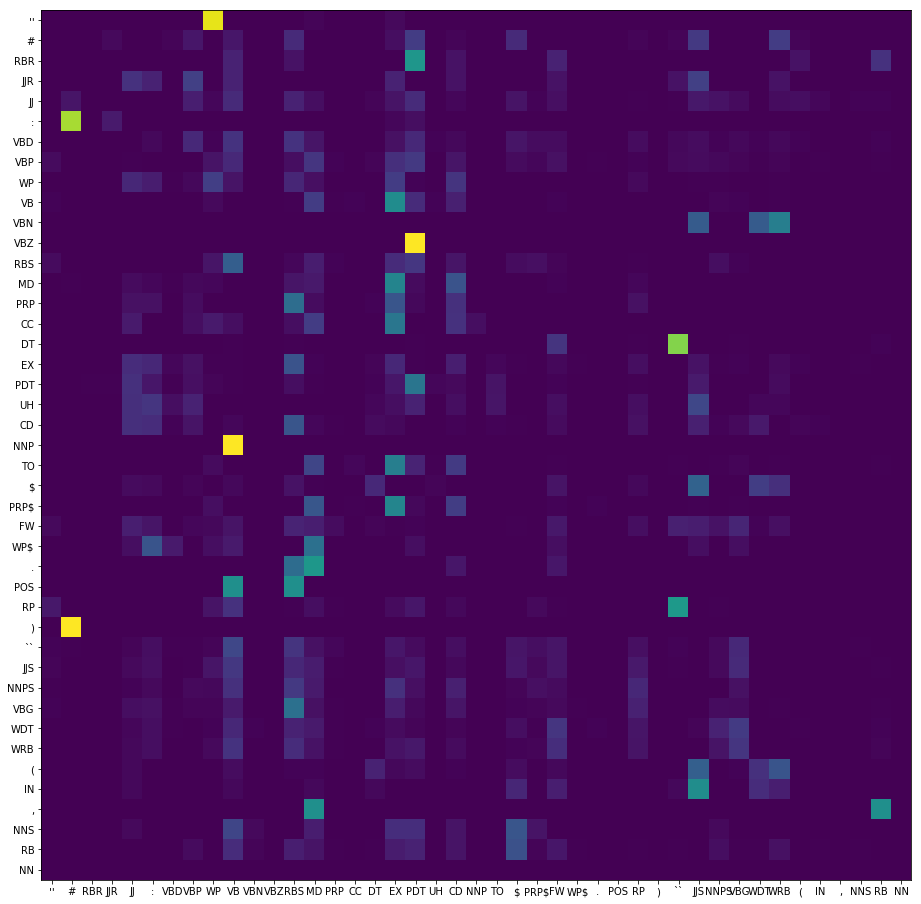
\includegraphics[width=0.6\textwidth]{images/tme1/transition_matrix.png}
    \caption{Matrice de transition}
    \label{img:tme1-transition-matrix}
\end{figure}

En test, nous obtenons une performance de 81\%, ce qui est meilleur que
l'approche précédente, sans post-traitement sur les mots inconnus.

La matrice de confusion est représentée sur la
\figref{img:tme1-confusion-matrix}. Nous pouvons observer qu'elle est proche
d'une matrice diagonale, ce qui permet de confirmer la qualité du modèle.

\begin{figure}[H]
	\center 
	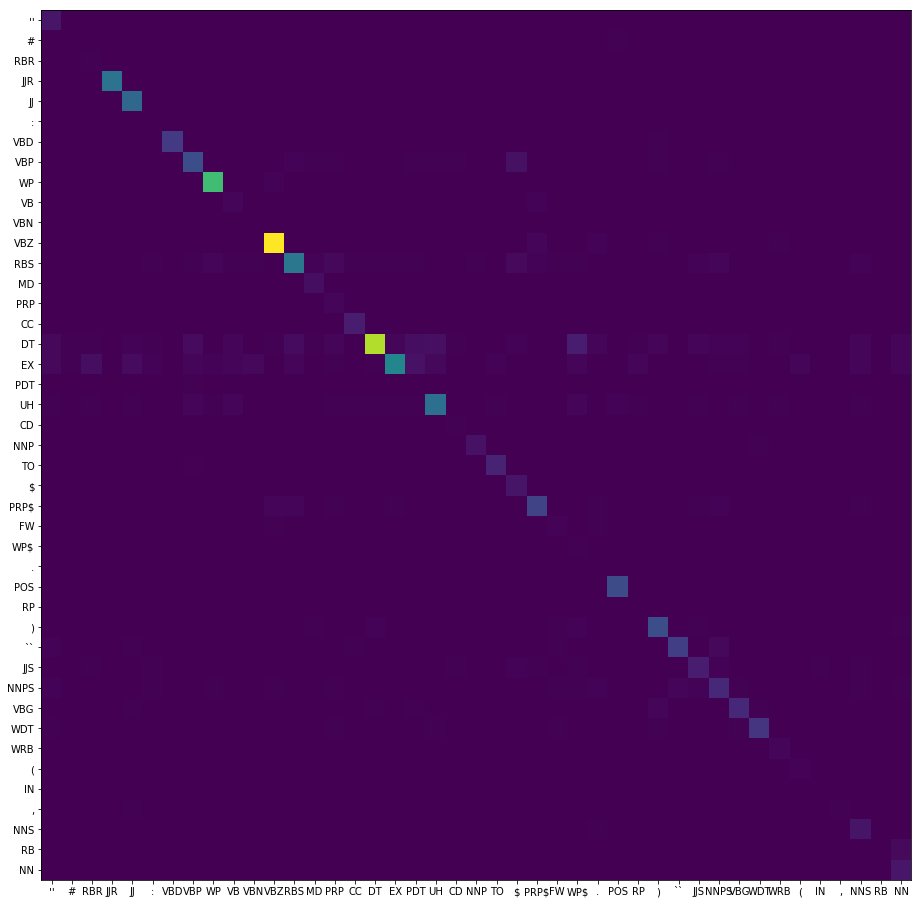
\includegraphics[width=0.6\textwidth]{images/tme1/confusion_matrix.png}
    \caption{Matrice de confusion}
    \label{img:tme1-confusion-matrix}
\end{figure}

Nous affichons également la matrice $\psi$ sur la \figref{img:tme1-psi-matrix}
obtenue par application de l'algorithme de Viterbi sur un document. Les colonnes
n'étant pas homogènes, nous pouvons voir l'intérêt de la modélisation
séquentielle.

\begin{figure}[H]
	\center 
	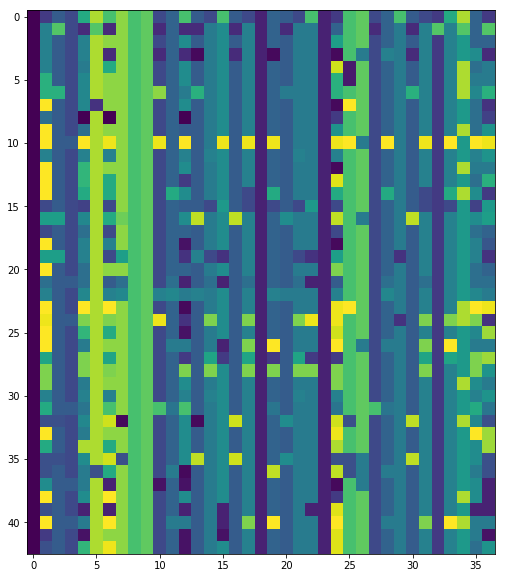
\includegraphics[width=0.5\textwidth]{images/tme1/psi_matrix.png}
    \caption{Matrice $\psi$}
    \label{img:tme1-psi-matrix}
\end{figure}

\subsection{Expériences dans nltk}

Nous prenons désormais en main la bibliothèque nltk \cite{nltk}, en particulier
l'objet \texttt{PerceptronTagger}, qui permet d'apprendre un Perceptron sur la
tâche de POS tagging.

Ce tagger fournit un taux de reconnaissance de 79.27\% sur le corpus de
test lorsque les mots sont considérés indépendamment les uns des autres, et de
91.82\% lorsqu'il est appliqué sur les phrases entières. 

Nous chargeons ensuite le POS tagger pré-entraîné de nltk afin de l'évaluer sur
le même corpus d'apprentissage. Son taux de reconnaissance est de 95.62\%
: ce POS tagger est donc meilleur que le précédent (notamment car il a été
entraîné sur bien plus de données).


\newpage
\section{Classification de documents}

Dans cette partie, nous menons des campagnes d'expériences afin d'optimiser les
performances de classification de documents. Nous considérons les deux tâches de
classification binaire suivantes :
\begin{itemize}
    \item Détection d'auteur : Chirac/Mitterrand (en français)
    \item Analyse de sentiments, représentation des textes (en anglais)
\end{itemize}

Nous utiliserons une chaîne de traitement standard, i.e. pré-traitements, mise
en forme et traitements. Sur chacune de ces tâches, nous cherchons à l'optimiser
:

\begin{itemize}
    \item trouver la bonne transformation des données textuelles,
    \item choisir le bon classifieur,
    \item optimiser ses paramètres,
    \item développer des outils de post-traitement et d'introspection des outils.
\end{itemize}

Nous choisissons de représenter nos données textuelles sous la forme BOW,
\emph{Bag of Words}. Chaque document sera représenté sous forme de vecteur, dans
lequel chaque dimension correspondra au nombre d'occurrences dans le document du
mot associé. L'objectif est alors d'effectuer les bons pré-traitements pour
construire un vocabulaire pertinent.

Le SVM linéaire étant un classifieur efficace et bien adapté au cas binaire,
nous choisissons d'utiliser le modèle \texttt{LinearSVC} de la librairie
Scikit-learn \cite{scikit}. Pour chacune des tâches, il sera optimisé par
validation croisée.

\subsection{Détection d'auteur : Chirac/Mitterrand}

Nous disposons d'un corpus de phrases étiquetées appartenant à J. Chirac et
F. Mitterrand. L'objectif est de développer un modèle qui prédise correctement
l'auteur de chaque phrase. Nous allons construire un classifieur binaire qui
assigne le label "C" (Chirac) ou "M" (Mitterrand) à une phrase. Comme le corpus
contient bien plus de phrases de J. Chirac que de F. Mitterrand, le score F1 sera
utilisé pour évaluer les performances de nos classifieurs.\\

Nous effectuons des expériences sur différentes transformations des données textuelles :
\begin{itemize}
    \item Unigrammes :
    \begin{itemize} 
        \item suppression des nombres
        \item suppression des nombres, des stopwords et des majuscules
        \item suppression des nombres, des stopwords, des accents, limitation de la taille du
            vocabulaire
    \end{itemize}
    \item Bi-grammes, suppression des nombres
    \item Tri-grammes :
    \begin{itemize}
        \item suppression des nombres
        \item suppression des nombres, des stopwords, des accents,
            limitation de la taille du vocabulaire
    \end{itemize}
\end{itemize}

\subsubsection{Unigrammes}

\textbf{Version 1 : suppression des nombres}

Nous considérons une première version qui ne prend pas en compte les nombres
mais n'effectue pas d'autre pré-traitement. Nous construisons un objet
\texttt{CountVectorizer} (de la bibliothèque Scikit-learn \cite{scikit}) à
partir des données d'apprentissage. Nous procédons ensuite à une validation
croisée en 10 folds pour trouver le meilleur paramétrage de notre modèle, en
faisant varier le terme de pénalité $C$ de $10^-4$ à $10^3$, par pas de $100$.
Le score F1 moyen obtenu en fonction de $C$ est tracé sur la
\figref{img:tme2-task1-v0}.

\begin{figure}[H]
	\center 
	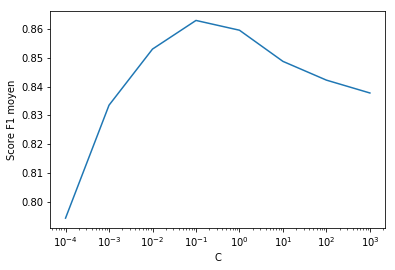
\includegraphics[width=0.6\textwidth]{images/tme2/task1_v0.png}
    \caption{Score $F1$ moyen en fonction de $C$}
    \label{img:tme2-task1-v0}
\end{figure}

Les meilleures performances sont obtenues avec $C=0.1$ : le score $F1$ moyen est
de $0.86$. En testant notre modèle avec ce paramétrage sur les données de test,
nous obtenons un score de $0.531$. 

Afin de comprendre d'où provient le score que notre modèle assigne à une phrase,
nous trions les éléments du vecteur de poids et récupérons les mots
correspondant aux $10$ premiers et $10$ derniers indices correspondant. Nous
obtenons ainsi les mots les plus polarisés. La \figref{tab:tme3-task1-v0-w}
contient les 10 mots du vocabulaire les plus représentatifs pour chaque
candidat.

\begin{table}[H]
\centering
\resizebox{0.9\textwidth}{!}{
\begin{tabular}{|c|c|}
    \hline
        Candidat & unigrammes \\
        \hline
        J. Chirac &  'propose', 'jeu', 'partager', 'insécurité', 'gagne', \\
        & 'partenariat', 'probablement', 'mondialisation', 'impressionné', 'euro'\\
        \hline
        F. Mitterrand & 'archives', 'soviétique', 'intelligences',
        'renégociation', 'cnrs', \\
        & 'sidérurgie', 'défauts', 'attendant', 'reçus', 'apprennent'\\
        \hline
\end{tabular}}
\caption{10 unigrammes les plus polarisés pour J. Chirac et F. Mitterrand}
\label{tab:tme3-task1-v0-w}
\end{table}

\textbf{Ajout de post-traitements}

Nous considérons désormais les prédictions de notre modèle, et faisons
l'hypothèse qu'une prédiction "M" apparaissant parmi plusieurs "C", et
vice-versa, est incorrecte. Nous remplaçons donc chacune de ces décisions par la
prédiction inverse : nous obtenons ainsi des groupes homogènes de "C" et "M".

NB : Ce post-traitement est utilisé pour l'évaluation sur le serveur. Comme nous
n'y avons malheureusement plus accès, nous ne pouvons pas afficher les scores
obtenus.


\textbf{Version 2 : suppression des nombres, des stopwords et des majuscules}

Afin d'enlever du dictionnaire des termes non pertinents, nous rajoutons à cette
première version la suppression des stopwords, i.e. les mots non significatifs,
et des majuscules. Comme précédemment, nous effectuons
une validation croisée afin d'optimiser notre modèle ; les résultats en termes
de score F1 sont tracés sur la \figref{img:tme2-task1-v1}.

\begin{figure}[H]
	\center 
	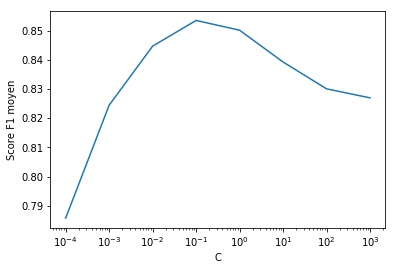
\includegraphics[width=0.6\textwidth]{images/tme2/task1_v1.png}
    \caption{Score $F1$ moyen en fonction de $C$}
    \label{img:tme2-task1-v1}
\end{figure}

En paramétrant notre SVM avec la valeur de $C$ ayant fourni le meilleur score en
apprentissage, i.e. $C=0.1$, nous obtenons une performance de $0.514$ en test.
Nous remarquons que ces pré-traitements dégradent légèrement les performances du
modèle. \\

\textbf{Version 3a : suppression des nombres, des stopwords, des accents,
limitation du vocabulaire à 10000 tokens}

Nous considérons maintenant un dictionnaire limité à $10000$ mots où les
nombres, les mots vides, et l'accentuation ne sont pas considérés. Les
performances produites lors de la validation croisée sont présentées sur la
\figref{img:tme2-task1-v2}.

\begin{figure}[H]
	\center 
	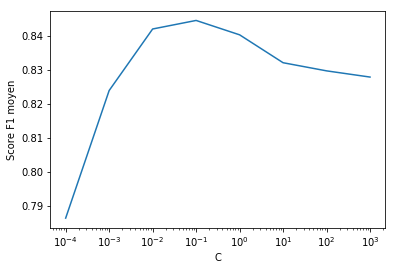
\includegraphics[width=0.6\textwidth]{images/tme2/task1_v2a.png}
    \caption{Score $F1$ moyen en fonction de $C$}
    \label{img:tme2-task1-v2}
\end{figure}

L'intervalle de valeurs des scores produits par ces modèles est
approximativement le même que les précédents. 

Les meilleurs résultats sont encore une fois obtenus avec $C=0.1$. En apprenant
notre SVM avec ce paramétrage, le score F1 sur le corpus de test est de $0.420$.
L'ajout de pré-traitements diminue nettement la performance du classifieur. \\

\textbf{Version 3b : suppression des nombres, des stopwords et des majuscules}

Nous effectuons les mêmes pré-traitements que dans la version précédente, en
rajoutant la stemmatisation des mots. Les scores obtenus lors
de l'optimisation du modèle sont présentés sur la \figref{img:tme2-task1-v1b}

\begin{figure}[H]
	\center 
	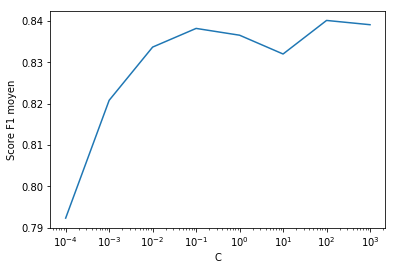
\includegraphics[width=0.6\textwidth]{images/tme2/task1_v2b.png}
    \caption{Score $F1$ moyen en fonction de $C$}
    \label{img:tme2-task1-v1b}
\end{figure}

Encore une fois, les scores obtenus prennent leurs valeurs dans un intervalle
semblable aux précédents.

Cependant, en paramétrant notre SVM sur la valeur optimale ($C=10^2$), les
performances en test chutent considérablement : nous obtenons un score $F1$ de
$0.157$. 


\subsubsection{Version 4 : Bigrammes}

Nous souhaitons observer l'impact des bi-grammes sur les performances de notre
modèle : au lieu de séparer chaque mot, nous prenons en compte les paires de
mots consécutifs. Nous ne gardons pas les nombres, mais n'effectuons pas d'autres
pré-traitements. La courbe du score F1 obtenu en apprentissage en fonction de
$C$ se trouve sur la \figref{img:tme2-task1-v3}. Ces résultats sont visiblement
meilleurs que ceux obtenus avec les unigrammes.

\begin{figure}[H]
	\center 
	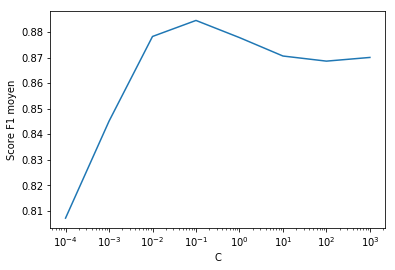
\includegraphics[width=0.6\textwidth]{images/tme2/task1_v3.png}
    \caption{Score $F1$ moyen en fonction de $C$}
    \label{img:tme2-task1-v3}
\end{figure}

En revanche, il n'y a pas de différence significative de performance sur les
données de test : le score $F1$ obtenu est de $0.515$. 

Afin d'évaluer qualitativement nos résultats, nous extrayons du modèle le
vecteur de poids correspondant. Les bigrammes les plus discriminants, pour
chaque candidat, se trouvent sur la \figref{tab:tme3-task1-v3-w}.

\begin{table}[H]
\centering
\resizebox{0.9\textwidth}{!}{
\begin{tabular}{|c|c|}
    \hline
        Candidat & bigrammes \\
        \hline
        J. Chirac & 'une solution', 'naturellement il', 'outre mer', \\
        & 'nos compatriotes', 'mesdames messieurs', 'vous remercie', \\
        &'crois pas', 'communauté internationale', 'la mondialisation', 'bien
        sûr' \\
        \hline
        F. Mitterrand & 'suite sur', 'date date', 'mais enfin', \\
        & 'solidarité économique', 'après tout', 'quelques autres',\\
        &'une façon', 'quand même', 'très bien', 'sont légion' \\
        \hline
\end{tabular}}
\caption{10 bigrammes les plus polarisés pour J. Chirac et F. Mitterrand}
\label{tab:tme3-task1-v4-w}
\end{table}

\subsubsection{Trigrammes}

Nous considérons à présent les tuples de trois mots consécutifs : les tri-grammes. \\

\textbf{Version 5 : Suppression des nombres}

Nous supprimons uniquement les nombres du dictionnaire. Les résultats obtenus
lors de la validation croisée sont présentés sur la \figref{img:tme2-task1-v4}.
Comme dans le cas des bi-grammes, les scores sont globalement meilleurs que ceux
obtenus en considérant les mots un par un.

\begin{figure}[H]
	\center 
	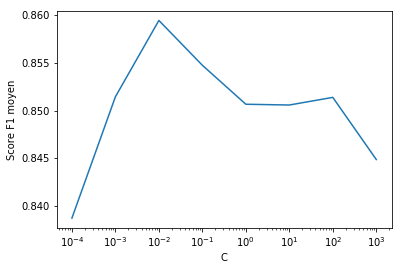
\includegraphics[width=0.6\textwidth]{images/tme2/task1_v4.png}
    \caption{Score $F1$ moyen en fonction de $C$}
    \label{img:tme2-task1-v4}
\end{figure}

Cependant, le modèle appris (avec $C=0.1$) sur le corpus d'apprentissage n'a pas
un bon pouvoir de généralisation : il génère un score $F1$ de $0.390$ sur les
données de test, ce qui est significativement pire que les résultats associés
aux unigrammes et bi-grammes. 

Comme précédemment, nous nous servons du vecteur de poids généré afin de
procéder à une analyse qualitative de notre classifieur. Les trigrammes les plus
employés par chaque candidat sont représentés sur la \figref{tab:tme3-task1-v4-w}.

\begin{table}[H]
\centering
\resizebox{0.7\textwidth}{!}{
\begin{tabular}{|c|c|}
    \hline
        Candidat & trigrammes \\
        \hline
        J. Chirac & 'est aussi une', 'de la mondialisation', \\
        &'dans notre pays', 'de union européenne', \\
        & 'que nous devons', 'plus que jamais', \\
        & 'la communauté internationale', 'tous les français', \\
        &'au service de', 'et messieurs les'\\
        \hline
        F. Mitterrand & 'en tout cas', 'etats unis amérique', \\
        & 'je me souviens', 'jepense que', \\
        & 'ici et là', 'il faut que', \\
        & 'de la communauté', 'je veux dire', \\
        & 'ce est pas', 'il faut bien' \\
        \hline
\end{tabular}}
\caption{10 trigrammes les plus polarisés pour J. Chirac et F. Mitterrand}
\label{tab:tme3-task1-v4-w}
\end{table}



\textbf{Version 6 : Suppression des nombres, des stopwords, des accents, limitation de la
taille du vocabulaire}

Nous limitons désormais la taille du vocabulaire à 10000 tokens et enlevons les
nombres, les mots vides, et l'accentuation. Les scores générés lors de la
validation croisée sont visualisés sur la \figref{img:tme2-task1-v5}.

\begin{figure}[H]
	\center 
	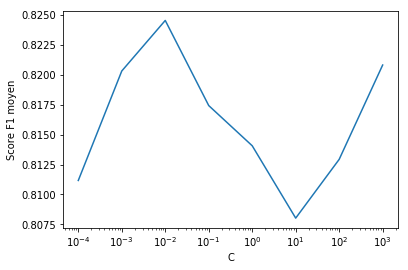
\includegraphics[width=0.6\textwidth]{images/tme2/task1_v5.png}
    \caption{Score $F1$ moyen en fonction de $C$}
    \label{img:tme2-task1-v5}
\end{figure}

En revanche, le modèle ne généralise pas correctement et produit un score $F1$ qui est
pire que celui obtenu avec les bi-grammes : il est de $0.224$. 

\subsubsection{Résumé}

Le \tabref{tab:tme2-task1-results} regroupe les scores avec chaque version sur
le corpus de test. 

\begin{table}[H]
\centering
\resizebox{0.8\textwidth}{!}{
\begin{tabular}{|*{8}{c|}}
    \hline
        Version & 1 & 2 & 3a & 3b & 4 & 5 & 6 \\
        \hline
        Score $F1$ en test & 0.531 & 0.514 & 0.420 & 0.157 & 0.515 & 0.390 & 0.224 \\

    \hline
\end{tabular}}
\caption{Score $F1$ obtenu sur le corpus de test pour chaque version}
\label{tab:tme2-task1-results}
\end{table}

Nous remarquons que l'ajout de pré-traitements (versions 2, 3a, 3b, et 6) dégrade
la qualité des classifieurs appris sur cette tâche : en effet, un auteur est
caractérisé par ses tournures de phrases, et celles-ci sont définies par des
termes supprimés par nos traitements. La stemmatisation, en particulier, fait
chuter les performances car il regroupe en une seule entité plusieurs termes
d'étiquettes morpho-syntaxiques souvent différentes (e.g. un verbe et un nom).
De plus, les résultats de Romain Ayres
\footnote{http://webia.lip6.fr/~guigue/wikihomepage/uploads/Course/Ayres2013.pdf}
montrent que les stopwords sont discriminants sur cette tâche.

Nous observons également des performances moins bonnes lorsque nous considérons
les n-grammes (version 4, 5 et 6). De plus, plus $n$ est grand, plus le modèle se dégrade en test.
En effet, comme le nombre de dimensions augmente très rapidement avec $n$, le
classifieur est vite sujet au sur-apprentissage. Intuitivement, nous pouvons
imaginer qu'il n'est pas pertinent de considérer des suites de trois mots
consécutifs étant donné leur faible fréquence d'apparition.

Afin d'extraire les topics de ces données, nous utilisons l'implémentation 
\subsection{Analyse de sentiments : polarité de revues}

Nous attaquons désormais une tâche d'analyse de sentiments : nous disposons d'un
ensemble de revues de films étiquetées en sentiments (positif/négatif) et
l'objectif est de pouvoir les prédire. Les classes étant équilibrées, nous
utilisons comme indicateur de performance le taux de reconnaissance.

Nous évaluerons nos modèles en fonction des mêmes traitements que pour la tâche
précédente. 

\subsubsection{Unigrammes}

\textbf{Version 1 : suppression des nombres}

Notre première version considère un vocabulaire construit sur l'ensemble
d'apprentissage où seulement les nombres ont été omis. Nous cherchons le
meilleur paramétrage de $C$ (dans le même intervalle que précédemment) par
validation croisée, et traçons les moyennes des taux de reconnaissance obtenus
pour chaque valeur de $C$ sur la \figref{img:tme2-task2-v0}. Nous pouvons
observer que le modèle perd en qualité lorsque $\alpha$ dépasse $10^{-2}$.

\begin{figure}[H]
	\center 
	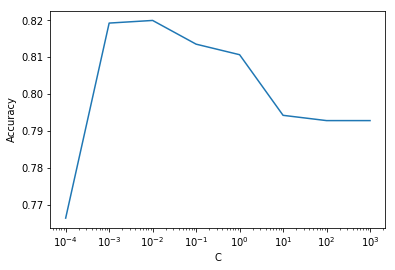
\includegraphics[width=0.6\textwidth]{images/tme2/task2_v0.png}
    \caption{Taux de reconnaissance moyen en fonction de $C$}
    \label{img:tme2-task2-v0}
\end{figure}

Nous paramétrons notre classifieur final, appris sur le corpus d'apprentissage
complet, avec la valeur de $C$ optimale, i.e.  $C=10**-3$. Sur les revues de
test, il fournit un taux de reconnaissance de $0.827$. 

Comme dans la tâche précédente, nous souhaitons connaître les mots les plus
discriminants afin de comprendre le score attribué à un document. La
\figref{tab:tme3-task2-v0-w} contient les mots du vocabulaire les plus
polarisés, récupérés grâce au vecteur de poids du classifieur précédent.

\begin{table}[H]
\centering
\resizebox{0.6\textwidth}{!}{
\begin{tabular}{|c|c|}
    \hline
        Sentiment & unigrammes \\
        \hline
        Négatif & 'bad', 'script', 'nothing', 'director', 'worst', \\
        & 'any', 'only', 'poor', 'plot', 'unfortunately'\\
        \hline
        Positif & 'also', 'memorable', 'perfectly', 'movies', 'well', \\
        & 'very', 'seen', 'quite', 'without', 'great' \\
        \hline
\end{tabular}}
\caption{20 mots les plus polarisés}
\label{tab:tme3-task2-v0-w}
\end{table}

À vue d'œil, ces résultats semblent cohérents : les termes \emph{bad},
\emph{worst}, \emph{poor} coïncident avec un sentiment négatif, et
\emph{perfectly}, \emph{well}, \emph{great}, avec un sentiment positif. \\

\textbf{Version 2 : suppression des nombres, des stopwords et des majuscules}

Dans cette deuxième version, nous supprimons du vocabulaire les stopwords ainsi
que les majuscules. La \figref{img:tme2-task2-v1} contient les taux de bonne
classification obtenus lors de la validation croisée.

\begin{figure}[H]
	\center 
	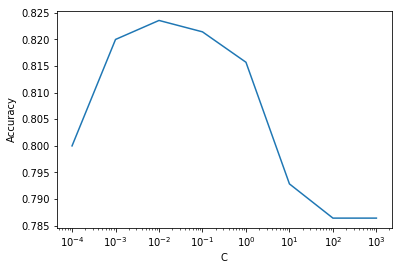
\includegraphics[width=0.6\textwidth]{images/tme2/task2_v1.png}
    \caption{taux de reconnaissance moyen en fonction de $C$}
    \label{img:tme2-task2-v1}
\end{figure}

L'intervalle des scores produits en apprentissage est très similaire au
précédent.

En paramétrant notre SVM avec $C=10**{-2}$, nous obtenons une performance de
$0.830$ en test. Ces pré-traitements améliorent légèrement les résultats. \\

\textbf{Version 3a : suppression des nombres, des stopwords, des accents,
limitation du vocabulaire à 10000 tokens}

Nous limitons la taille du dictionnaire à $10000$ termes, et supprimons les
nombres, les stopwords, et l'accentuation. La validation croisée fournit les
scores tracés sur la \figref{img:tme2-task2-v2a}.

\begin{figure}[H]
	\center 
	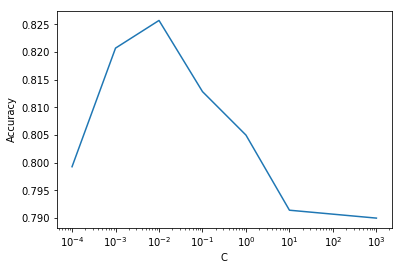
\includegraphics[width=0.6\textwidth]{images/tme2/task2_v2a.png}
    \caption{taux de reconnaissance moyen en fonction de $C$}
    \label{img:tme2-task2-v2a}
\end{figure}

L'intervalle de valeurs des résultats est approximativement le même que les
précédents. 

Sur les données de test et avec $C=0.1$, nous obtenons un taux de bonne
classification de $0.822$. Les pré-traitements considérés diminuent légèrement
les performances du modèle par rapport aux précédents. \\

\textbf{Version 3b : suppression des nombres, des stopwords, des majuscules et
stemmatistion}

Nous effectuons les mêmes pré-traitements que dans la version précédente, en
rajoutant la stemmatisation des mots. Les scores obtenus lors
de l'optimisation du modèle sont présentés sur la \figref{img:tme2-task2-v2b}.

\begin{figure}[H]
	\center 
	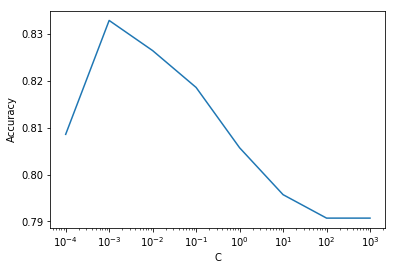
\includegraphics[width=0.6\textwidth]{images/tme2/task2_v2b.png}
    \caption{taux de reconnaissance moyen en fonction de $C$}
    \label{img:tme2-task2-v2b}
\end{figure}

Encore une fois, les scores obtenus lors de la validation croisée sont
similaires à ceux générés par les versions précédentes.

Sur les revues de test et avec $C=10**-3$, nous obtenons un taux de
reconnaissance de $0.848$.

\subsubsection{Version 4 : Bi-grammes}

Nos dictionnaires sont désormais constitués de bi-grammes. Nous enlevons les
nombres, mais ne considérons pas d'autres pré-traitements. La
\figref{img:tme2-task2-v3} contient l'évolution du taux de reconnaissance
en fonction de $C$, lors de la validation croisée.

\begin{figure}[H]
	\center 
	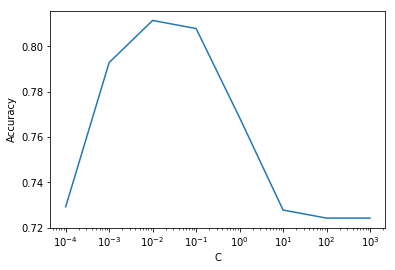
\includegraphics[width=0.6\textwidth]{images/tme2/task2_v3.png}
    \caption{Taux de reconnaissance moyen en fonction de $C$}
    \label{img:tme2-task2-v3}
\end{figure}

Cette fois-ci, les résultats obtenus lors de la phase d'optimisation semblent
moins bons que les précédents : les scores sont compris entre $0.72$ et $0.82$.

De même, l'évaluation sur les données de test (avec $C=10**{-2}$) fournit un
taux de reconnaissance de $0.802$, ce qui est légèrement moins bon que les
versions précédentes. 

Comme pour le cas des unigrammes, nous trions le vecteur de poids associé au
modèle afin de récupérer les $20$ bigrammes les plus polarisés du vocabulaire.
Les résultats se trouvent sur la \figref{tab:tme3-task2-v3}.

\begin{table}[H]
\centering
\resizebox{0.7\textwidth}{!}{
\begin{tabular}{|c|c|}
    \hline
        Sentiment & bigrammes \\
        \hline
        Négatif & 'the worst', 'have been', 'the only', 'supposed to', 'at
        least', \\
        & 'should have', 'it just', 'to be', 'but the', 'the script' \\
        \hline
        Positif & 'but it', 'very well', 'even if', 'due to', 'the right', \\
        & 'as well', 'he is', 'as the', 'is very', 'the best' \\
        \hline
\end{tabular}}
\caption{20 bigrammes les plus polarisés}
\label{tab:tme3-task2-v3-w}
\end{table}

Cette fois-ci, exceptés \emph{the worst}, \emph{very well} et \emph{the best},
les termes obtenus sont moins facilement interprétables que les unigrammes de la
\figref{tab:tme3-task2-v1-w}. \\

\subsubsection{Tri-grammes}

Nous considérons à présent les tri-grammes. \\

\textbf{Version 5 : Suppression des nombres}

Le seul pré-traitement effectué dans cette version est la suppression des
nombres. Nous traçons les résultats obtenus lors de la validation croisée sur la
\figref{img:tme2-task2-v4}.

\begin{figure}[H]
	\center 
	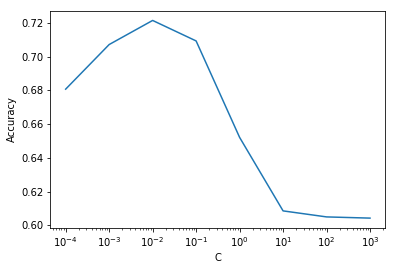
\includegraphics[width=0.6\textwidth]{images/tme2/task2_v4.png}
    \caption{Taux de reconnaissance moyen en fonction de $C$}
    \label{img:tme2-task2-v4}
\end{figure}

Les performances chutent significativement : le taux de reconnaissance
prend ses valeurs dans l'intervalle $[0.60, 0.72]$. 

De même, le score calculé sur les revues de test (avec $C=10**{-2}$) est de
$0.711$ ; ce qui est pire que celui obtenu avec les bi-grammes. 

Comme précédemment, nous souhaitons visualiser les mots les plus polarisés selon
ce classifieur ; les résultats sont présentés sur la
\figref{tab:tme3-task2-v4-w}.

\begin{table}[H]
\centering
\resizebox{0.7\textwidth}{!}{
\begin{tabular}{|c|c|}
    \hline
        Sentiment & trigrammes \\
        \hline
        Négatif & 'could have been', 'of the worst', 'supposed to be', \\
        & 'in this movie', 'would have been', 'to work with', \\
        & 'is supposed to', 'of the movie', 'in the movie', 'to be funny'\\
        \hline
        Positif & 'some of the', 'but it is', 'one of his', \\
        & 'is able to', 'is one of', 'in the world', \\
        & 'as well as', 'one of the', 'the film is', 'of the best'\\
        \hline
\end{tabular}}
\caption{20 trigrammes les plus polarisés}
\label{tab:tme3-task2-v4-w}
\end{table}

Le lien entre les trigrammes obtenus et la polarité correspondante est encore
plus floue en considérant les trigrammes ; ce résultat qualitatif est cohérent
avec la diminution du taux de reconnaissance observée lors du passage de
bigrammes à trigrammes. \\

\textbf{Version 6 : Suppression des nombres, des stopwords, des accents, limitation de la
taille du vocabulaire}

Nous limitons désormais la taille du vocabulaire à 10000 tokens et supprimons
les nombres, les mots vides, et l'accentuation. L'évolution du taux de bonne
classification généré lors de la validation croisée se trouve sur la
\figref{img:tme2-task2-v5}.

\begin{figure}[H]
	\center 
	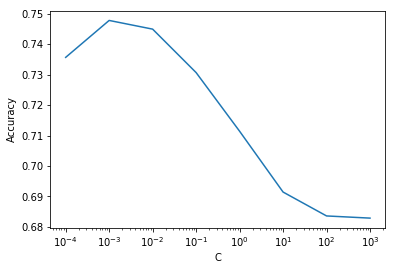
\includegraphics[width=0.6\textwidth]{images/tme2/task2_v5.png}
    \caption{taux de reconnaissance moyen en fonction de $C$}
    \label{img:tme2-task2-v5}
\end{figure}

Les scores sont meilleurs que ceux de la version précédente : ils sont compris
entre $0.68$ et $0.75$.

En test, ces pré-traitements permettent d'obtenir de meilleurs résultats : le
taux de reconnaissance obtenu est de $0.757$.

\subsubsection{Résumé}

Le \tabref{tab:tme2-task2-results} regroupe les résultats obtenus avec chaque
version sur les revues de test. 

\begin{table}[H]
\centering
\resizebox{0.8\textwidth}{!}{
\begin{tabular}{|*{8}{c|}}
    \hline
        Version & 1 & 2 & 3a & 3b & 4 & 5 & 6 \\
        \hline
        Taux de reconnaissance en test (\%) & 82.7 & 83.0 & 82.2 & 84.8 & 80.2 & 71.1 &  75.7\\
    \hline
\end{tabular}}
\caption{taux de reconnaissance obtenu sur le corpus de test pour chaque version}
\label{tab:tme2-task2-results}
\end{table}

Sur cette tâche, les meilleurs résultats sont obtenus avec un vocabulaire
composés d'unigrammes, dans lequel les termes sont stemmatisés et les nombres,
les stopwords, et les majuscules sont omis (version 3b). De plus, les
pré-traitements ajoutés sur les trigrammes (version 6) semble également
améliorer les performances. Nous constatons donc la différence entre la tâche de
détection d'auteur et celle d'analyse de sentiments en termes de pré-traitements
: contrairement à la tâche précédente, la polarité d'un texte n'est pas
discriminée par des mots vides ou certaines étiquettes morpho-syntaxiques. 

\newpage
\section{Sémantique et catégorisation thématique}

Dans cette partie, nous étudions l'apprentissage d'une sémantique et la
classification non supervisée de documents. Nous travaillons dans un premier
temps avec les données \emph{Associated Press}, non étiquetées, puis dans un
second temps avec le dataset étiqueté \emph{Reuters}. L'objectif est d'en
extraire des topics pertinents.

\subsection{Catégorisation thématique sur les données \emph{Associated Press}}

Nous considérons les données \emph{Associated Press}, qui correspondent à de
courts articles non étiquetés. 

\subsubsection{Extraction de topics}

Les données sont mises sous forme vectorielle, en omettant les stopwords, les
nombres, ainsi que les termes apparaissant avec une fréquence inférieure à
$10**{-2}$ ou supérieure à $0.3$. 

Afin d'extraire les topics de ces données, nous utilisons l'implémentation de
Scikit-learn \cite{scikit} de l'algorithme LDA (\emph{Latent Dirichlet
Allocation}). La \figref{img:tme3-vis-5} contient les 30 mots les plus
pertinents de la troisième thématique, lorsque nous fixons le nombre de clusters
à $n=5$. Ces termes définissent vraisemblablement une thématique liée à la
Guerre Froide. 

\begin{figure}[H]
	\center 
	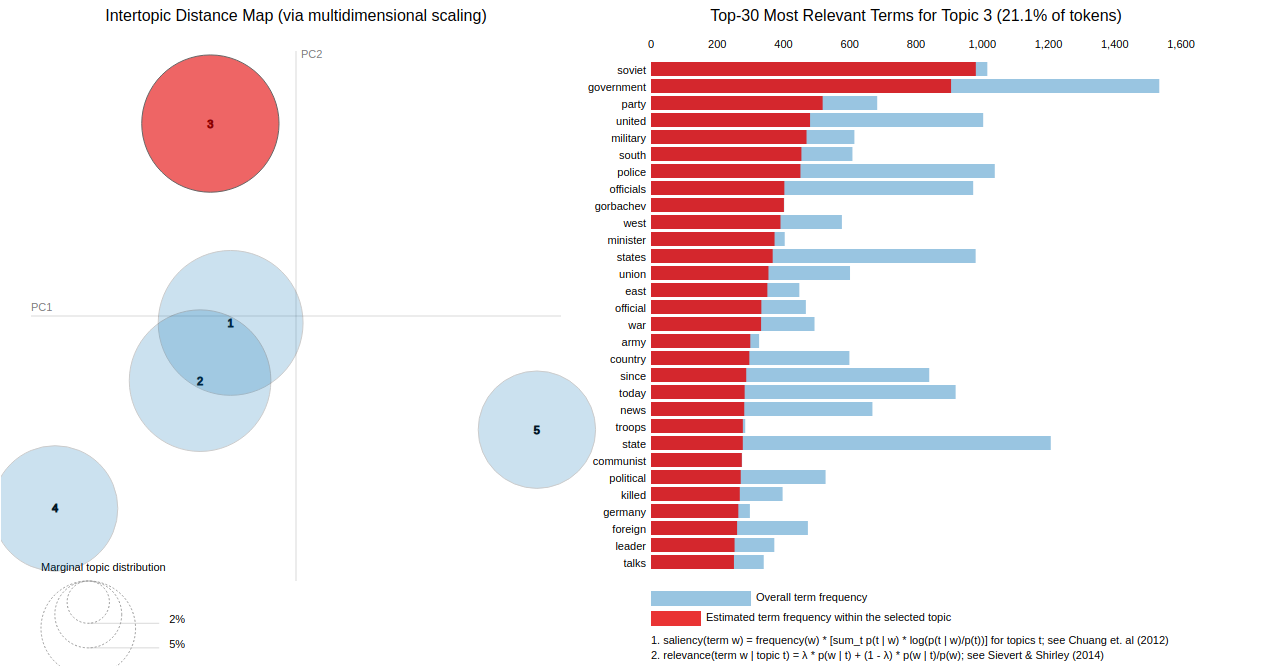
\includegraphics[width=1.2\textwidth]{images/tme3/vis_5.png}
    \caption{Visualisation des 5 clusters obtenus par LDA}
    \label{img:tme3-vis-5}
\end{figure}

Il est également possible de trouver ces clusters "à la main", i.e. sans passer
par les outils de visualisation. Nous extrayons de la décomposition LDA la
matrice $p(W|z)$, qui représente la distribution des mots $w$ pour chaque topic
$z$. Pour chaque $z$, les mots $w$ sont ensuite triés selon $p(w|z)$, dans
l'ordre décroissant. Nous récupérons ensuite les $20$ premiers de chaque
cluster. Les résultats sont présentés sur la \figref{tab:tme3-topic-words}.

\begin{table}[H]
\centering
\resizebox{0.9\textwidth}{!}{
\begin{tabular}{|c|c|}
    \hline
        Topic & 20 premiers mots triés\\
        \hline
        1 & 'say' 'women' 'get' 'night' 'health'\\
        & 'water' 'fire' 'died' 'show' 'world' \\
        & 'life' 'center' 'city' 'day' 'home' \\
        &'family' 'hospital' 'like' 'children' 'old' \\
        \hline
        2 &  'exchange' 'rates' 'cents' 'york' 'share'\\
        & 'price' 'trading' 'higher' 'rose' 'trade' \\
        & 'sales' 'dollar' 'oil' 'company' 'prices' \\
        & 'stock' 'market' 'billion' 'million' 'percent'\\
        \hline
        3 & 'think' 'support' 'going' 'budget' 'defense' \\
        & 'democratic' 'national' 'states' 'bill' 'senate' \\
        & 'administration' 'congress' 'committee' 'percent' 'state' \\
        & 'reagan' 'campaign' 'dukakis' 'house' 'bush'\\
        \hline
        4  & 'today' 'since' 'country' 'army' 'war'\\
        & 'official' 'east' 'union' 'states' 'minister'\\
        & 'west' 'gorbachev' 'officials' 'police' 'south' \\
        & 'military' 'united' 'party' 'government' 'soviet' \\
        \hline
        5  & 'law' 'prison' 'charges' 'government' 'office' \\
        & 'trial' 'workers' 'company' 'city' 'million' \\
        & 'attorney' 'judge' 'department' 'drug' 'officials' \\
        & 'case' 'state' 'federal' 'police' 'court' \\
    \hline
\end{tabular}}
\caption{20 premiers mots de chaque topic triés selon $p(w|z)$ décroissant}
\label{tab:tme3-topic-words}
\end{table}

Notons que les termes obtenus par cette méthode ne correspondent pas
complètement à ceux de la visualisation. En effet, cette dernière met en avant
les mots les plus saillants de chaque cluster, i.e. ceux qui apparaissent
beaucoup dans ce cluster mais peu ailleurs. 

\subsubsection{Inférence}

Nous souhaitons désormais inférer sur un nouveau document : à quel topic
correspond-il le plus ? \\

Nous considérons le document suivant : 

\texttt{Arij is sentenced to 10 years of prison due to heroin consumption.
According to NBC, she is reportedly not a \ consumer but a dealer}. \\

En appliquant la méthode
\texttt{sklearn.decomposition.LatentDirichletAllocation} sur le vecteur $x$ du
document, qui équivaut au produit scalaire entre $x$ et la matrice des
paramètres variationnels de la décomposition LDA, nous obtenons la distribution
de probabilités sur les topics suivante :

\texttt{[0.11621487, 0.39956597, 0.01830722, 0.01837959, 0.44753235]} \\

Ce vecteur indique que le topic le plus vraisemblable pour le document est le
5ème, lié, entre autres, à la \emph{loi}, la \emph{prison} et la \emph{drogue}.
Les résultats sont donc cohérents. Il est donc possible, à partir de la
décomposition LDA, de construire un modèle associant à un texte le topic le plus
pertinent.

Le corpus \emph{Associated Press} n'étant pas étiqueté, nous ne pouvons évaluer
que qualitativement les résultats obtenus.

\subsubsection{Catégorisation thématique sur les données \emph{Reuters}}

Afin d'avoir une évaluation quantitative de nos résultats, nous traitons le
dataset étiqueté \emph{Reuters}, qui comporte 90 topics. 

Nous utilisons comme indicateur de qualité des clusters créés la \emph{pureté}.
Pour la calculer, chaque cluster est assigné au topic le plus fréquent dans ce
cluster, puis l'on compte le nombre de documents correctement classés, que l'on
divise par le nombre total de documents. Formellement, en posant $\Omega =
\{\omega_1,...,\omega_K\}$ l'ensemble des clusters, et $C = \{c_1,...,c_J\}$
l'ensemble des classes :

\begin{equation} 
    purity(\Omega, C) = \frac{1}{n} \sum_{k} \max_{j}|\omega_k \cap c_j|
\label{eq:purity}
\end{equation}

Nous reprenons le code de \cite{reuters} afin de récupérer le dataset
\emph{Reuters}. Nous apprenons un modèle LDA à partir de ces données, en fixant
le nombre de topics à définir à $90$, i.e. autant qu'en contient le dataset, et
le nombre maximum d'itérations à $50$. 

En implémentant l'\eqref{eq:purity} et en l'appliquant sur cette décomposition
LDA, nous obtenons une pureté de $0.61$. \\ 

%\newpage
%\section{Représentation vectorielle des mots et documents}

\newpage
\printbibliography
\end{document}
